\documentclass[thesis.tex]{subfiles}

\begin{document}

\begin{align}
  \beta^{-}\ \text{decay}&:    &   n\ &\longrightarrow\ p + e^{-} + \bar{\nu}_{e} \\
  \beta^{+}\ \text{decay}&:    &   p\ &\longrightarrow\ n + e^{+} + \nu_{e} \\
  \text{Electron capture}&:  &   p + e^{-}\ &\longrightarrow\ n + \nu_{e}
\end{align}

\begin{table}
  \centering
  \begin{tabular}{ l @{\hskip 50pt} l @{\hskip 50pt} l } \hline
    Decay Type     & \Delta J = J_{F} - J_{I} & \pi_{F}\pi_{I} \\ \hline\hline
    Fermi          & 0                         & +1 \\
    Gamow-Teller   & 1    (J_{F}=0\ \text{or}\ J_{I}=0)   & +1 \\
    Gamow-Teller   & 0,1  (J_{F}>0\ \text{and}\ J_{I}>0)  & +1 \\ \hline
  \end{tabular}
  \caption{Single-particle states and their quantum numbers and their energies from Eq.~(\ref{eq:pairingsp}). The degeneracy for every quantum number $p$ is equal to 2 due to the two possible spin values.}
  \label{tab:pairingmodelsp}
\end{table}

\begin{figure}
  \centering
  \begin{subfigure}{0.5\linewidth}
    \centering
    \hspace{1.1cm}
    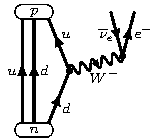
\includegraphics[height=3.5cm]{betadecay/BetaDecay-figure0.pdf}
  \end{subfigure}
  \hspace{-0.25\linewidth}
  \begin{subfigure}{0.5\linewidth}
    \centering
    \hspace{1.1cm}
    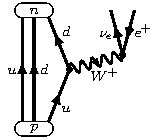
\includegraphics[height=3.5cm]{betadecay/BetaDecay-figure1.pdf}
  \end{subfigure}
\end{figure}

\begin{figure}
  \centering
  \begin{subfigure}{0.5\linewidth}
    \centering
    \hspace{1.1cm}
    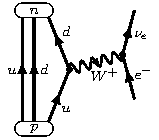
\includegraphics[height=3.5cm]{betadecay/BetaDecay-figure2.pdf}
  \end{subfigure}
  \hspace{-0.225\linewidth}
  \begin{subfigure}{0.5\linewidth}
    \centering
    \hspace{1.1cm}
    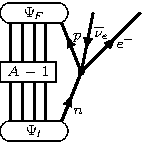
\includegraphics[height=3.5cm]{betadecay/BetaDecay-figure3.pdf}
  \end{subfigure}
\end{figure}

\begin{figure}
  \centering
  \begin{subfigure}{0.5\linewidth}
    \centering
    \hspace{1.0cm}
    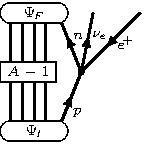
\includegraphics[height=3.5cm]{betadecay/BetaDecay-figure4.pdf}
  \end{subfigure}
  \hspace{-0.175\linewidth}
  \begin{subfigure}{0.5\linewidth}
    \centering
    \hspace{1.0cm}
    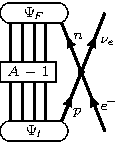
\includegraphics[height=3.5cm]{betadecay/BetaDecay-figure5.pdf}
  \end{subfigure}
\end{figure}



\section{Sum Rules}

\begin{gather}
  \sum_{F} \left[ B_{F_{-}}^{I,F} - B_{F_{-}}^{I,F} \right] = \sum_{F} \left[ \lvert \bra{F}\sum_{i}\tau_{i}^{-}\ket{I} \rvert^{2} - \lvert \bra{F}\sum_{i}\tau_{i}^{+}\ket{I} \rvert^{2} \right] \notag \\
  = \sum_{F} \left[ \bra{I}\sum_{i}\tau_{i}^{+}\ket{F}\bra{F}\sum_{i}\tau_{i}^{-}\ket{I} - \bra{I}\sum_{i}\tau_{i}^{-}\ket{F}\bra{F}\sum_{i}\tau_{i}^{+}\ket{I} \right] \notag \\
  = \bra{I} (\sum_{i}\tau_{i}^{+}) (\sum_{j}\tau_{j}^{-}) - (\sum_{i}\tau_{i}^{-}) (\sum_{j}\tau_{j}^{+}) \ket{I} = \bra{I} 2\sum_{i}\tau_{i}^{z} \ket{I} = \left( N_{I} - Z_{I} \right)
\end{gather}

\begin{gather}
  \sum_{F} \left[ B_{GT_{-}}^{I,F} - B_{GT_{-}}^{I,F} \right] = \sum_{F,\mu} \left[ \lvert \bra{F}\sum_{i}\sigma_{i}^{\mu}\tau_{i}^{-}\ket{I} \rvert^{2} - \lvert \bra{F}\sum_{i}\sigma_{i}^{\mu}\tau_{i}^{+}\ket{I} \rvert^{2} \right] \notag \\
  = \sum_{F,\mu} \left[ \bra{I}\sum_{i}\sigma_{i}^{\mu}\tau_{i}^{+}\ket{F}\bra{F}\sum_{i}\sigma_{i}^{\mu}\tau_{i}^{-}\ket{I} - \bra{I}\sum_{i}\sigma_{i}^{\mu}\tau_{i}^{-}\ket{F}\bra{F}\sum_{i}\sigma_{i}^{\mu}\tau_{i}^{+}\ket{I} \right] \notag \\
  = \sum_{\mu} \left[ \bra{I} (\sum_{i}\sigma_{i}^{\mu}\tau_{i}^{+}) (\sum_{j}\sigma_{i}^{\mu}\tau_{j}^{-}) - (\sum_{i}\sigma_{i}^{\mu}\tau_{i}^{-}) (\sum_{j}\sigma_{i}^{\mu}\tau_{j}^{+}) \ket{I} \right] \notag \\
  = \sum_{\mu} \left[ \bra{I} \sum_{i}\sigma_{i,\mu}^{2}\left( \tau_{i,+}\tau_{i,-} - \tau_{i,-}\tau_{i,+} \right) \ket{I} \right] = 3\ \bra{I} \sum_{i}\left( \tau_{i,+}\tau_{i,-} - \tau_{i,-}\tau_{i,+} \right) \ket{I} \notag \\
  = 3\ \bra{I} 2\sum_{i}\tau_{i}^{z} \ket{I} = 3\left( N_{I} - Z_{I} \right)
\end{gather}

\begin{gather}
  \sum_{F} \left[ B_{F_{-}}^{I,F} - B_{F_{-}}^{I,F} \right] = \left( N_{I} - Z_{I} \right) \\
  \sum_{F} \left[ B_{GT_{-}}^{I,F} - B_{GT_{-}}^{I,F} \right] = 3\left( N_{I} - Z_{I} \right)
\end{gather}

\end{document}
